\section{Non-linear Kalman filtering}

\subsection{a}

Part a and b have lots of pictures, I listed them and discuss together.

\begin{figure}[H]
 \centering
 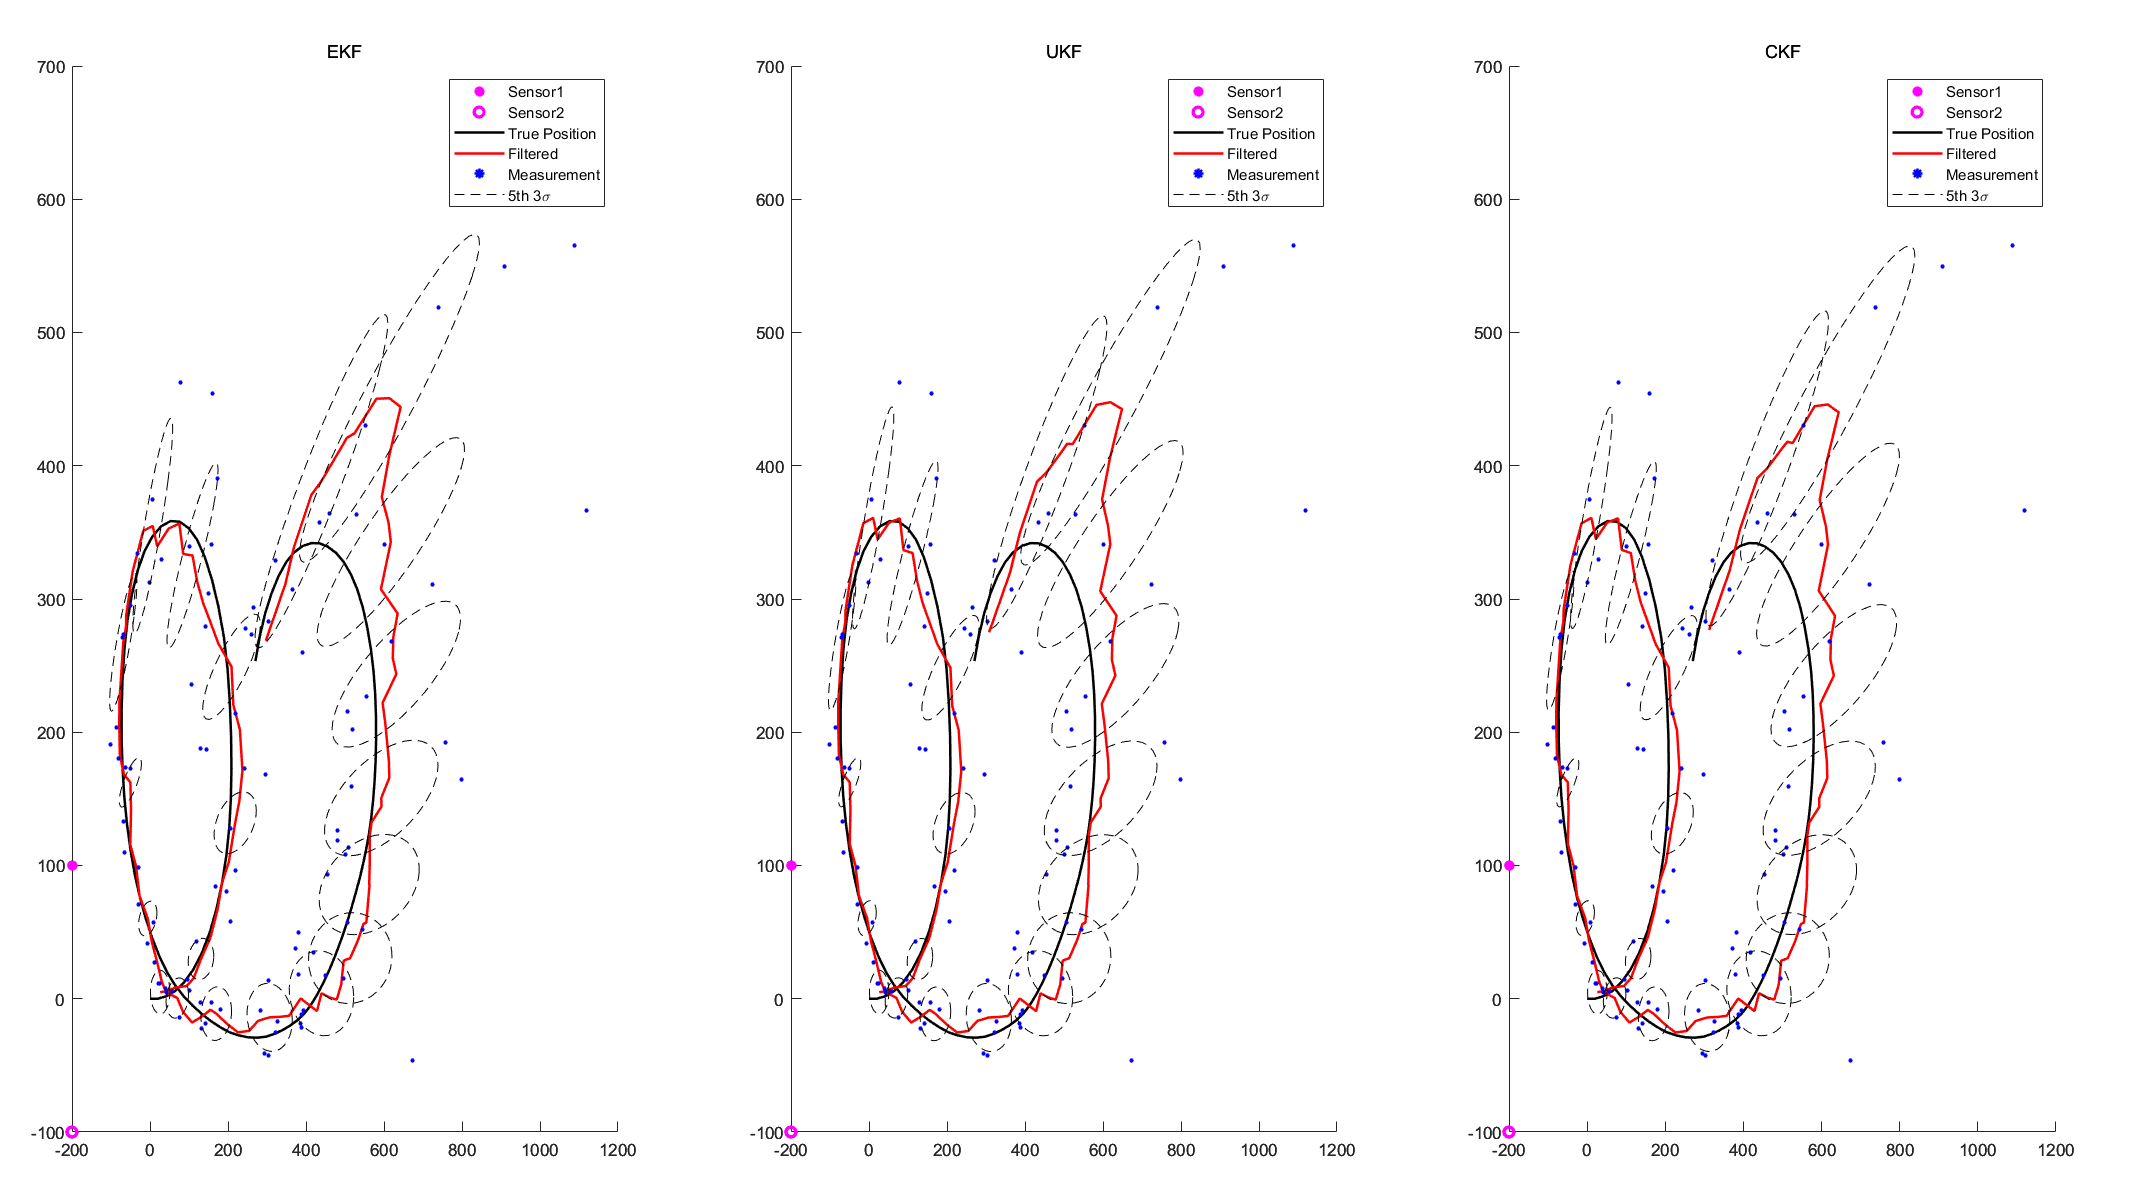
\includegraphics[width=0.95\textwidth]{images/normala.png}
 \caption{Normal Case}
 \label{normal}
\end{figure}


\begin{figure}[H]
 \centering
 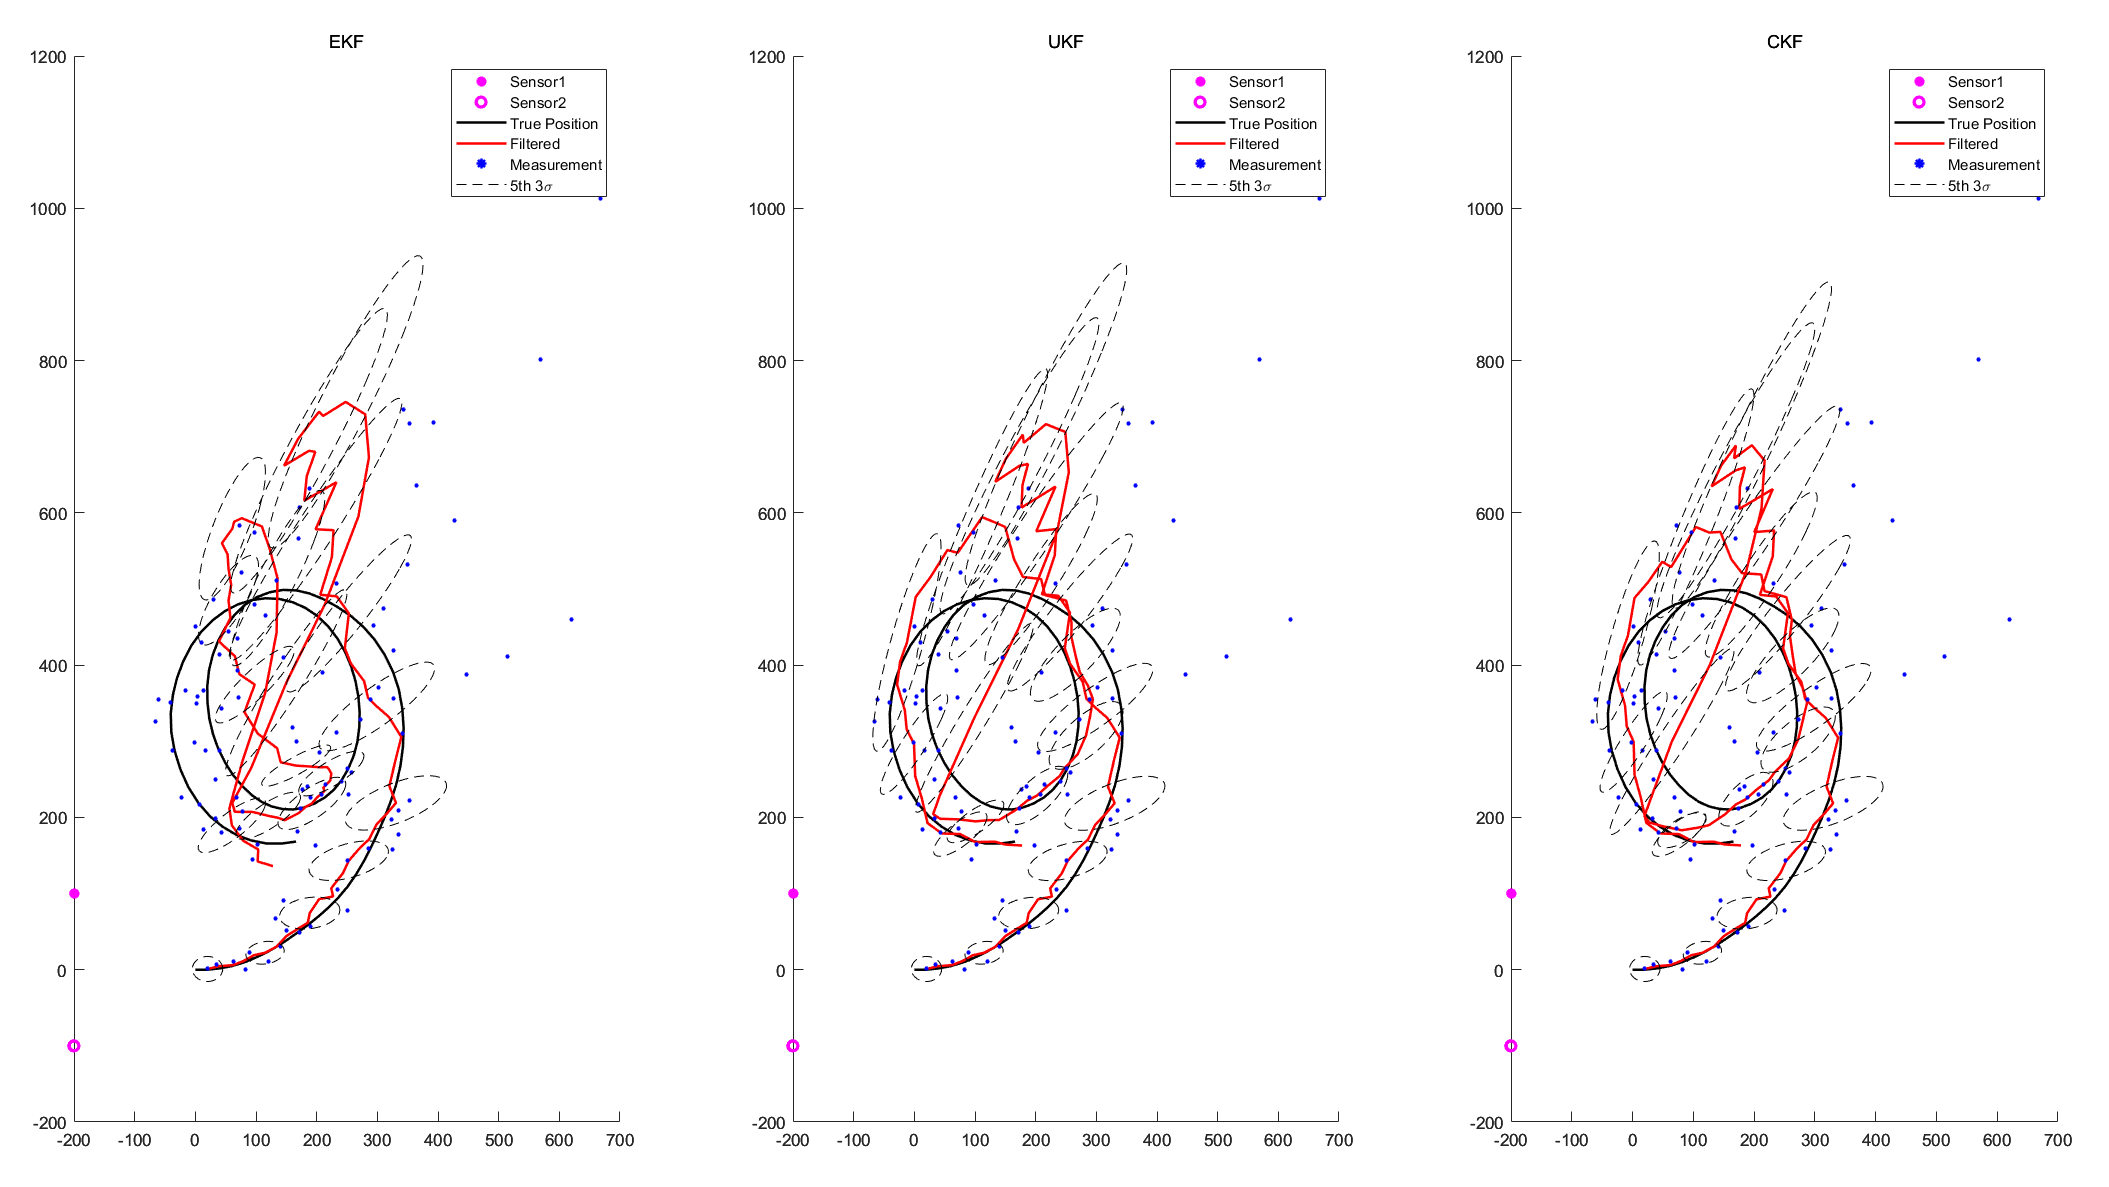
\includegraphics[width=0.95\textwidth]{images/case1.png}
 \caption{Extreme Situation (all bad)}
 \label{allbad}
\end{figure}

\begin{figure}[H]
 \centering
 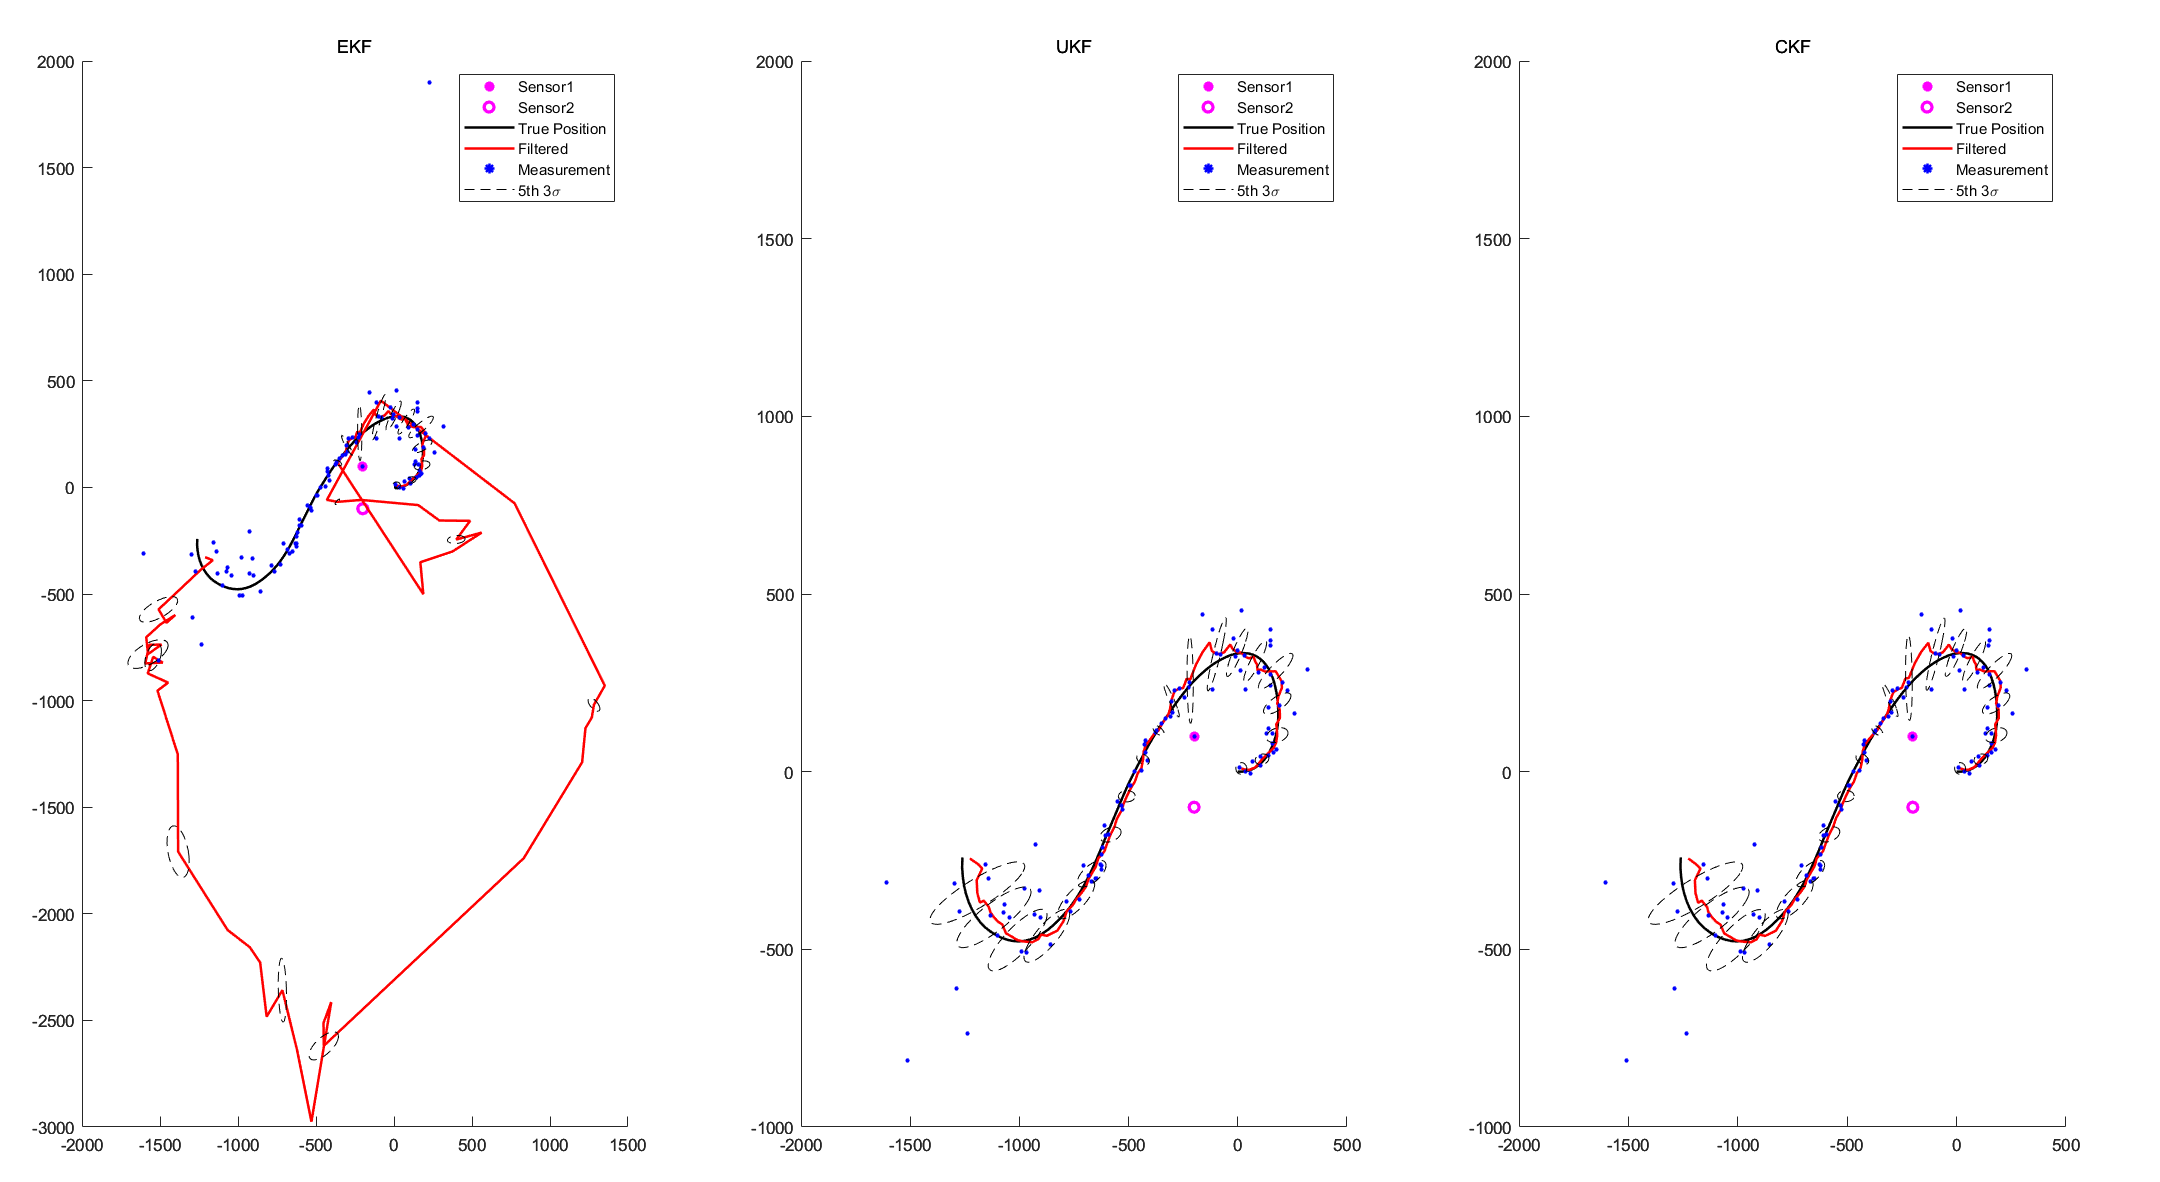
\includegraphics[width=0.95\textwidth]{images/extremea.png}
 \caption{Extreme Situation (EKF bad)}
 \label{EKFbad}
\end{figure}

\subsection{b}

\begin{figure}[H]
 \centering
 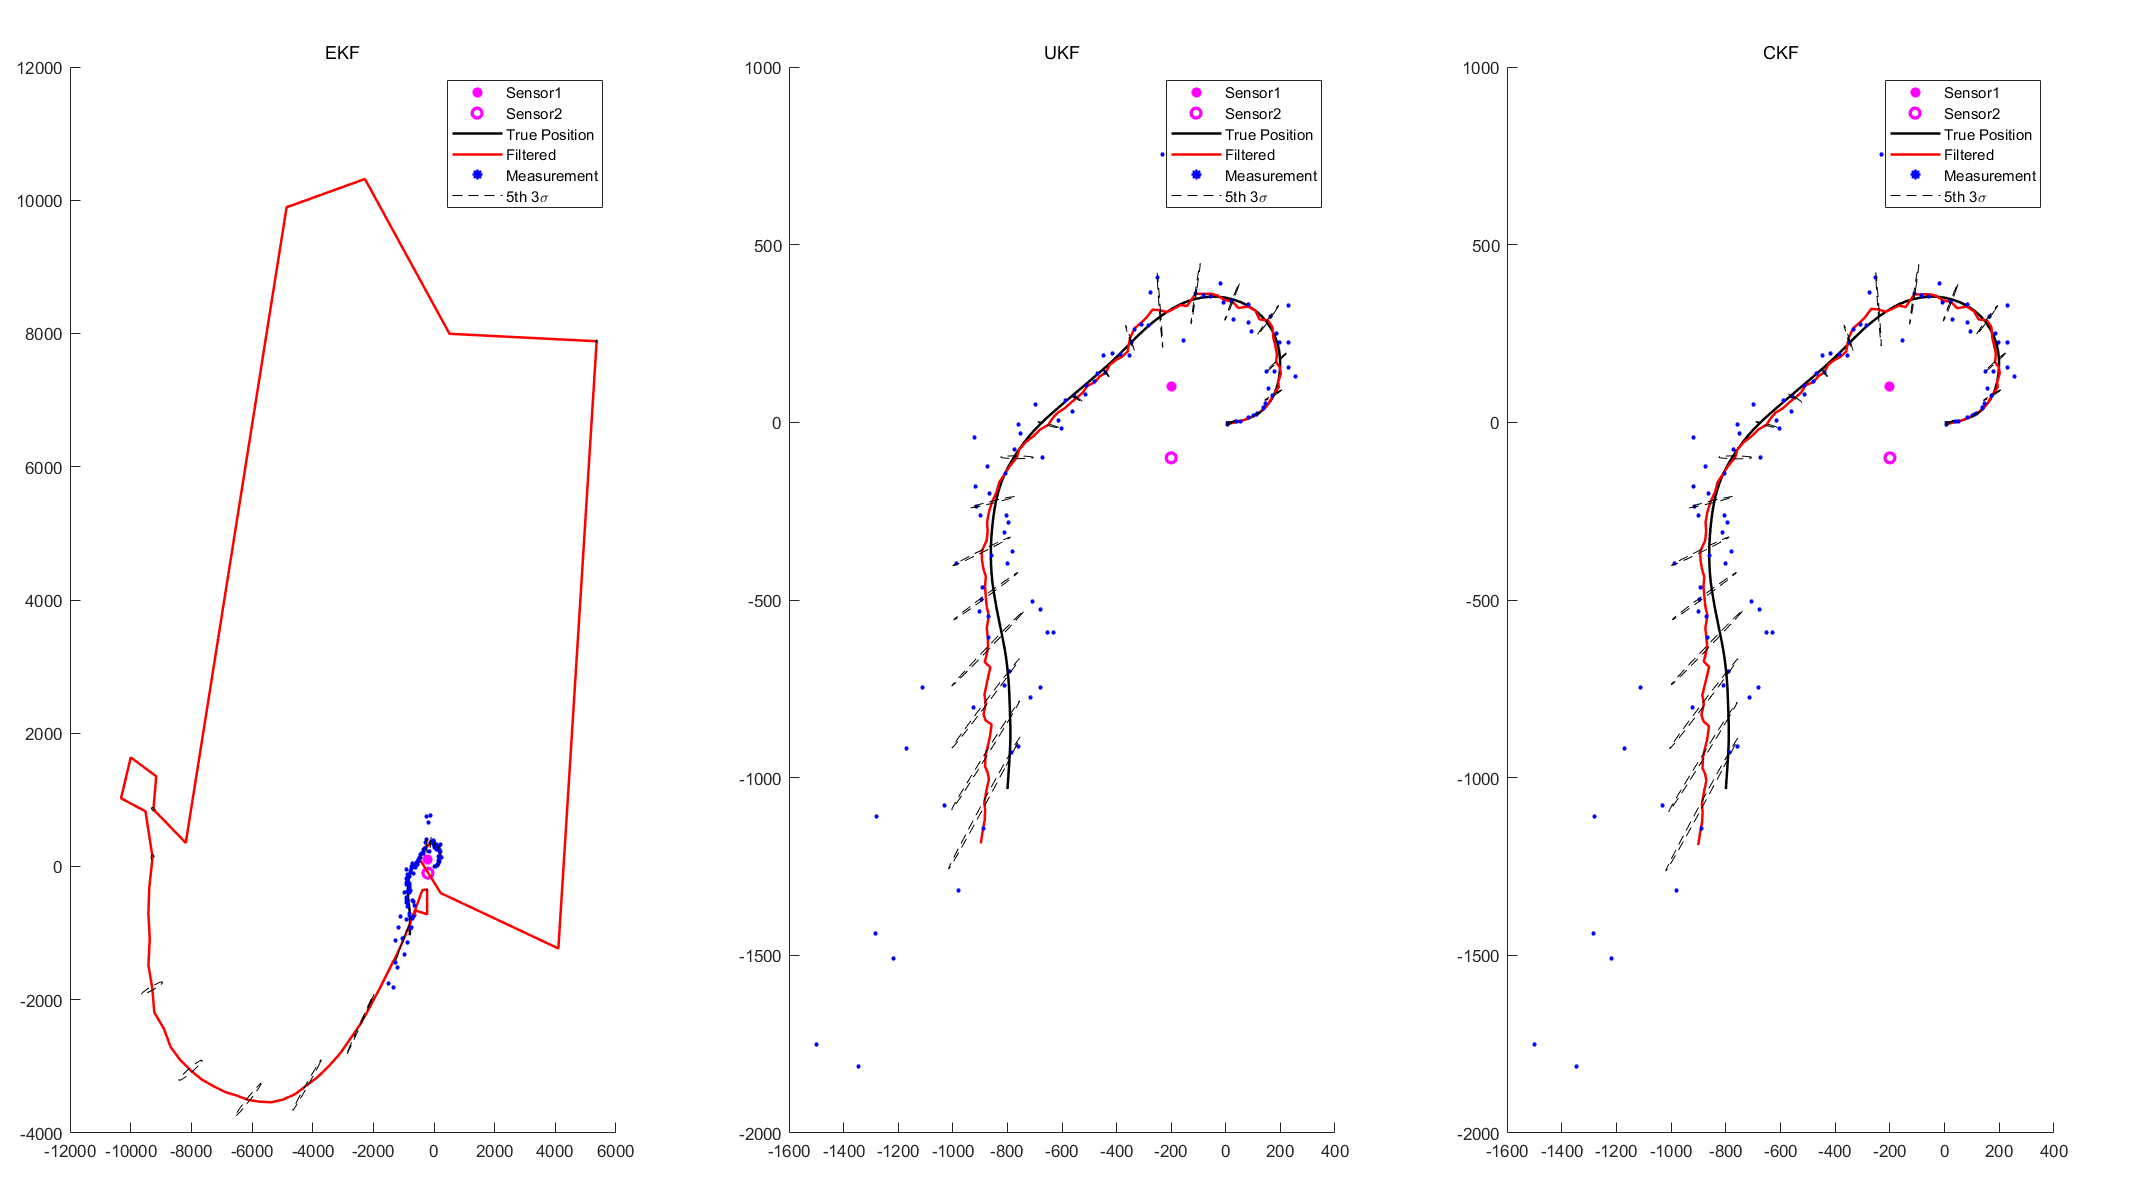
\includegraphics[width=0.95\textwidth]{images/extreme.png}
 \caption{Extreme Case 2}
 \label{extremecase2}
\end{figure}

\begin{figure}[H]
 \centering
 \includegraphics[width=0.95\textwidth]{images/Normalcase3.png}
 \caption{Normal Case 3}
 \label{2b}
\end{figure}

\subsection{discuss a\&b}

For this question, I tried a very large number of times. In the vast majority of cases, there is no significant difference between EKF and UKF/CKF, it achieves tracking very well, and its covariance is not significantly larger compared to the other two, and only in a few cases can be distinguished by the naked eye, like in figure \ref{allbad}.

The covariance is well represented by the unvertainty, can be seen in Figure \ref{normal}.

All methods are poor when the two trajectories are nearly coincident, showed in \ref{allbad}

The failure of the EKF can be observed when the car surrounds the sensor at a relatively close distance. This is because at very close distances to the sensor, as if two points were taken on a circle of small radius to connect the lines to represent the arc between them, the nonlinear of the car is so severe that the EKF fails. These cases showed in \ref{EKFbad} and \ref{extremecase2}

To be honest, although the extreme situation will fail, in my experience, the reliability of the EKF is amazing.

\subsection{c}

Upon the figures, I print the mean and covariance of the estimation errors. In this way it can be much more clear to evaluate the quality of the filter.

\begin{figure}[H]
 \centering
 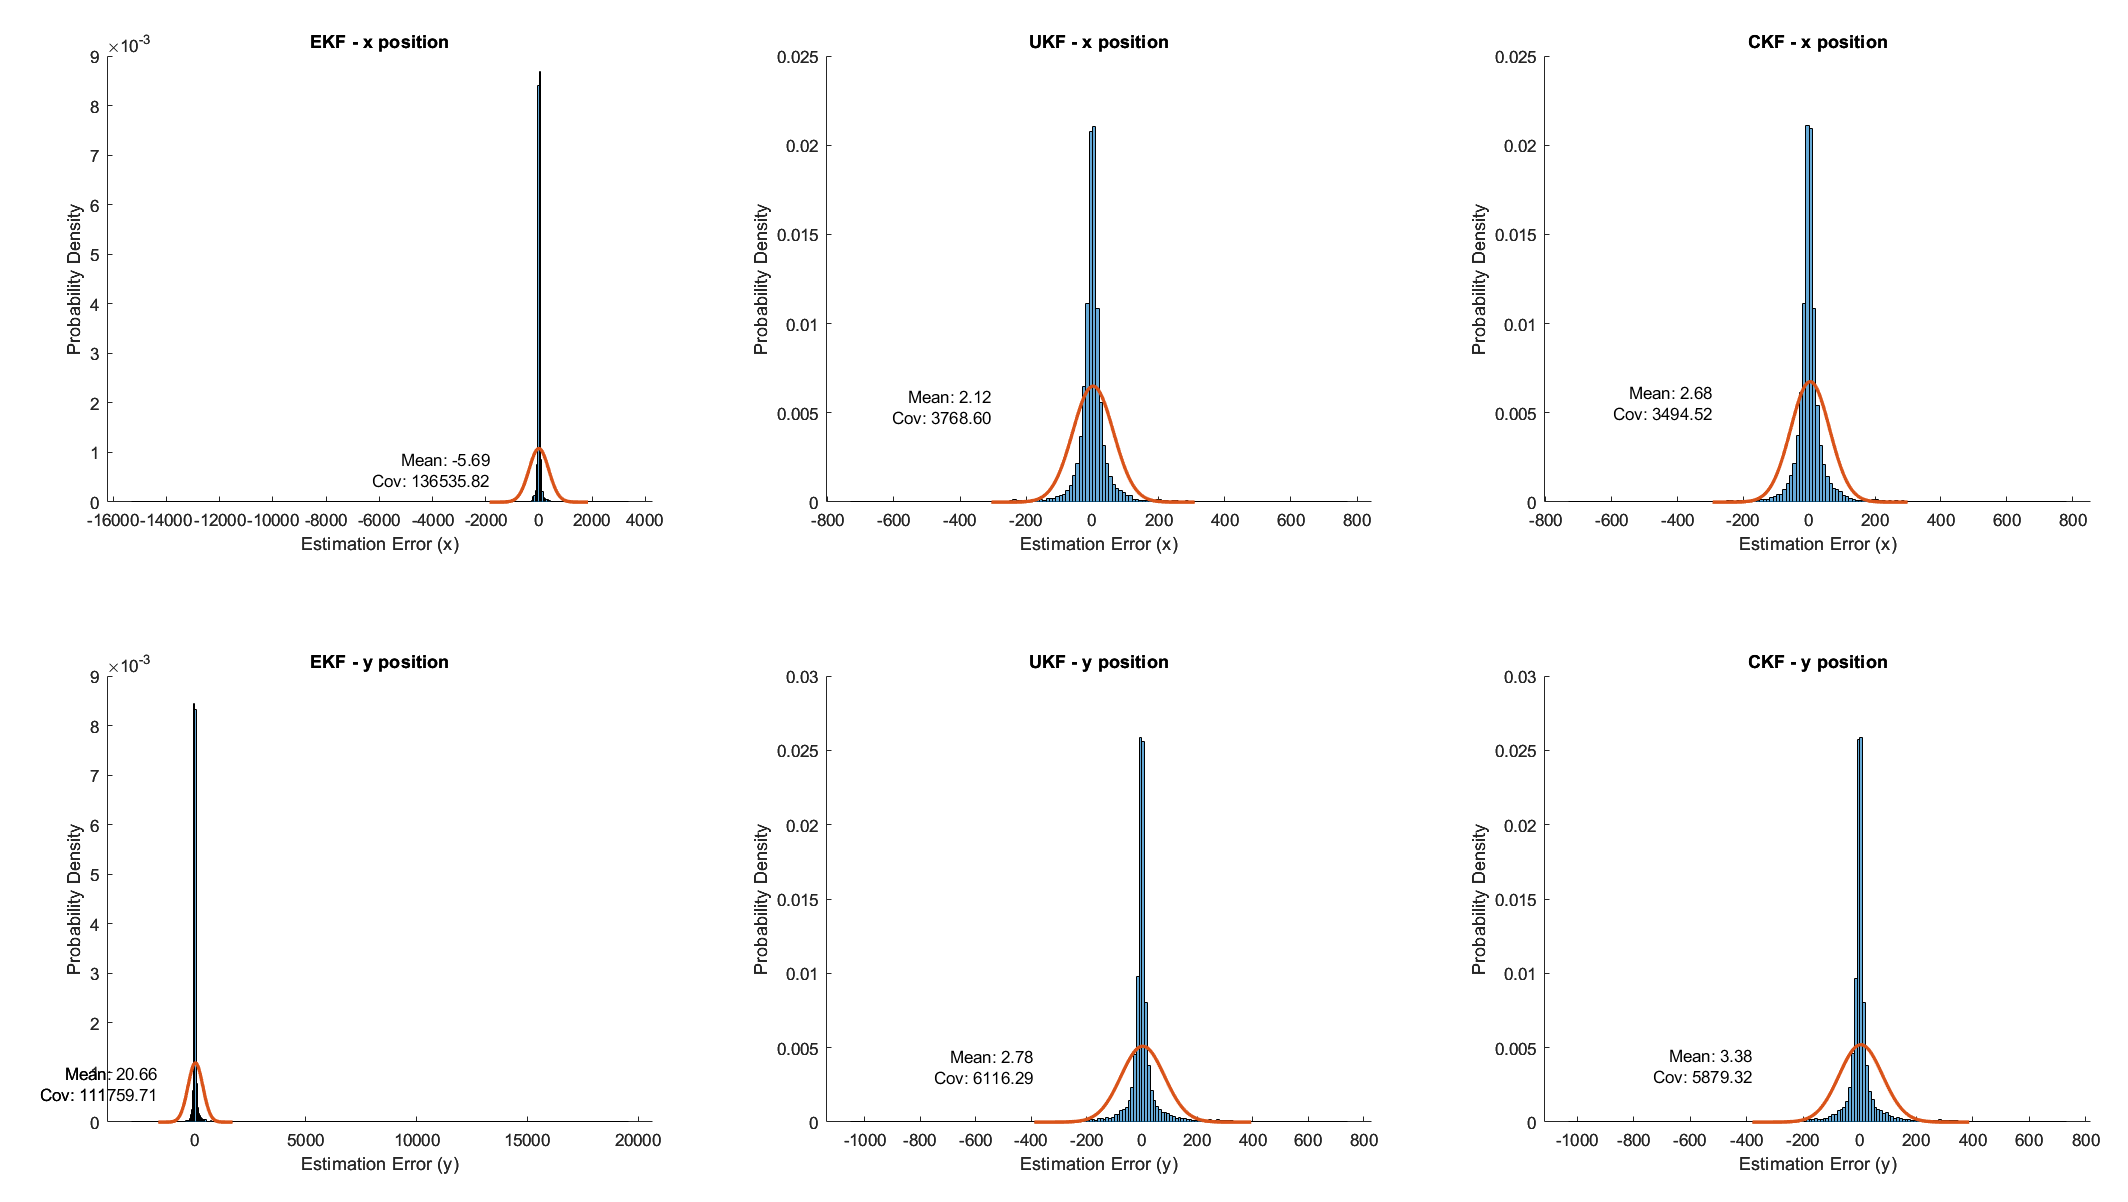
\includegraphics[width=0.95\textwidth]{images/hiscase1.png}
 \caption{Case 1}
 \label{c1}
\end{figure}

\begin{figure}[H]
 \centering
 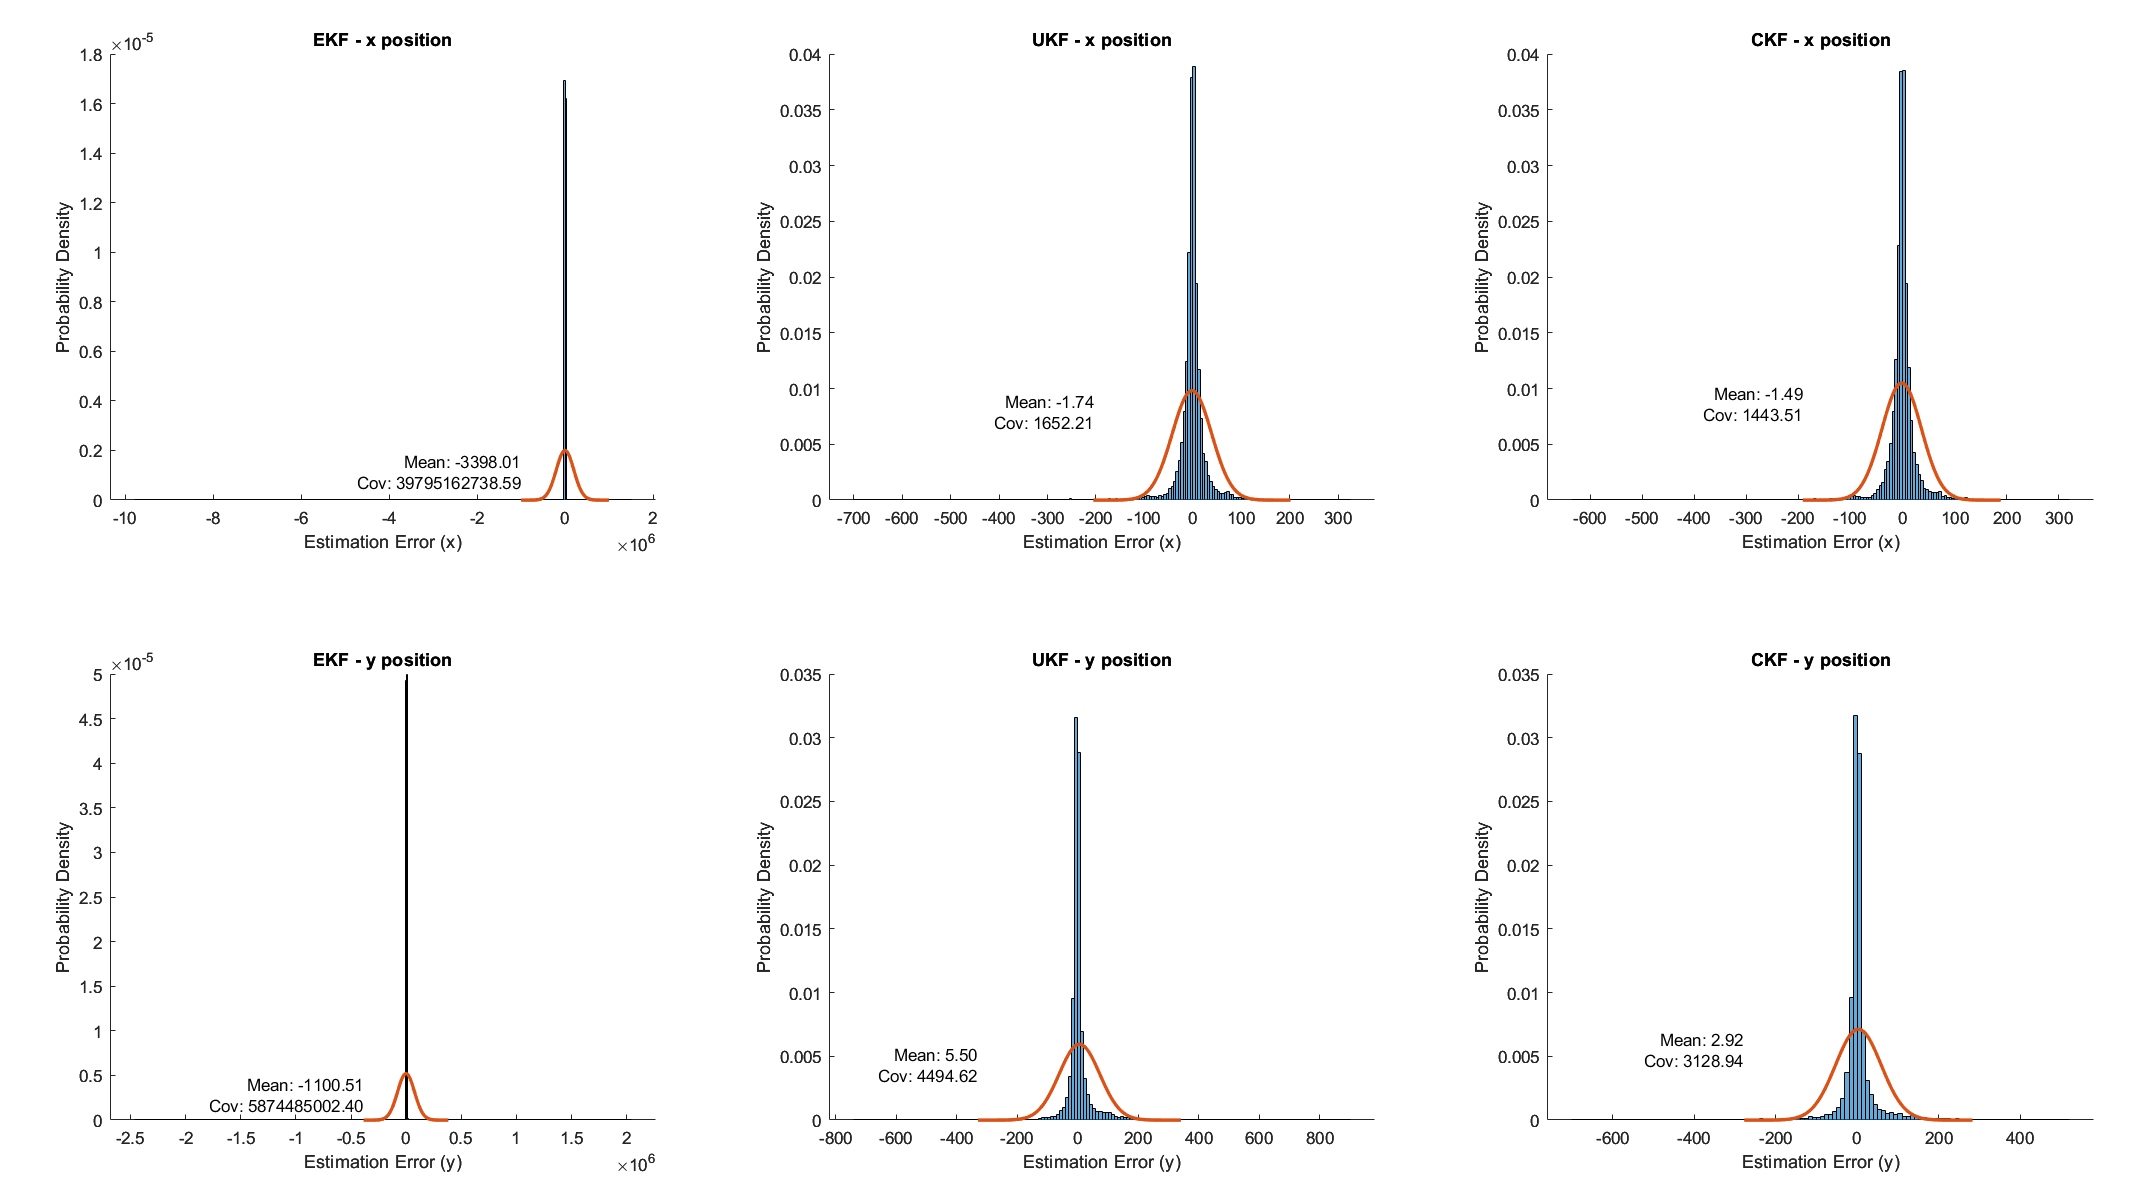
\includegraphics[width=0.95\textwidth]{images/hiscase2.png}
 \caption{Case 2}
 \label{c2}
\end{figure}

\begin{figure}[H]
 \centering
 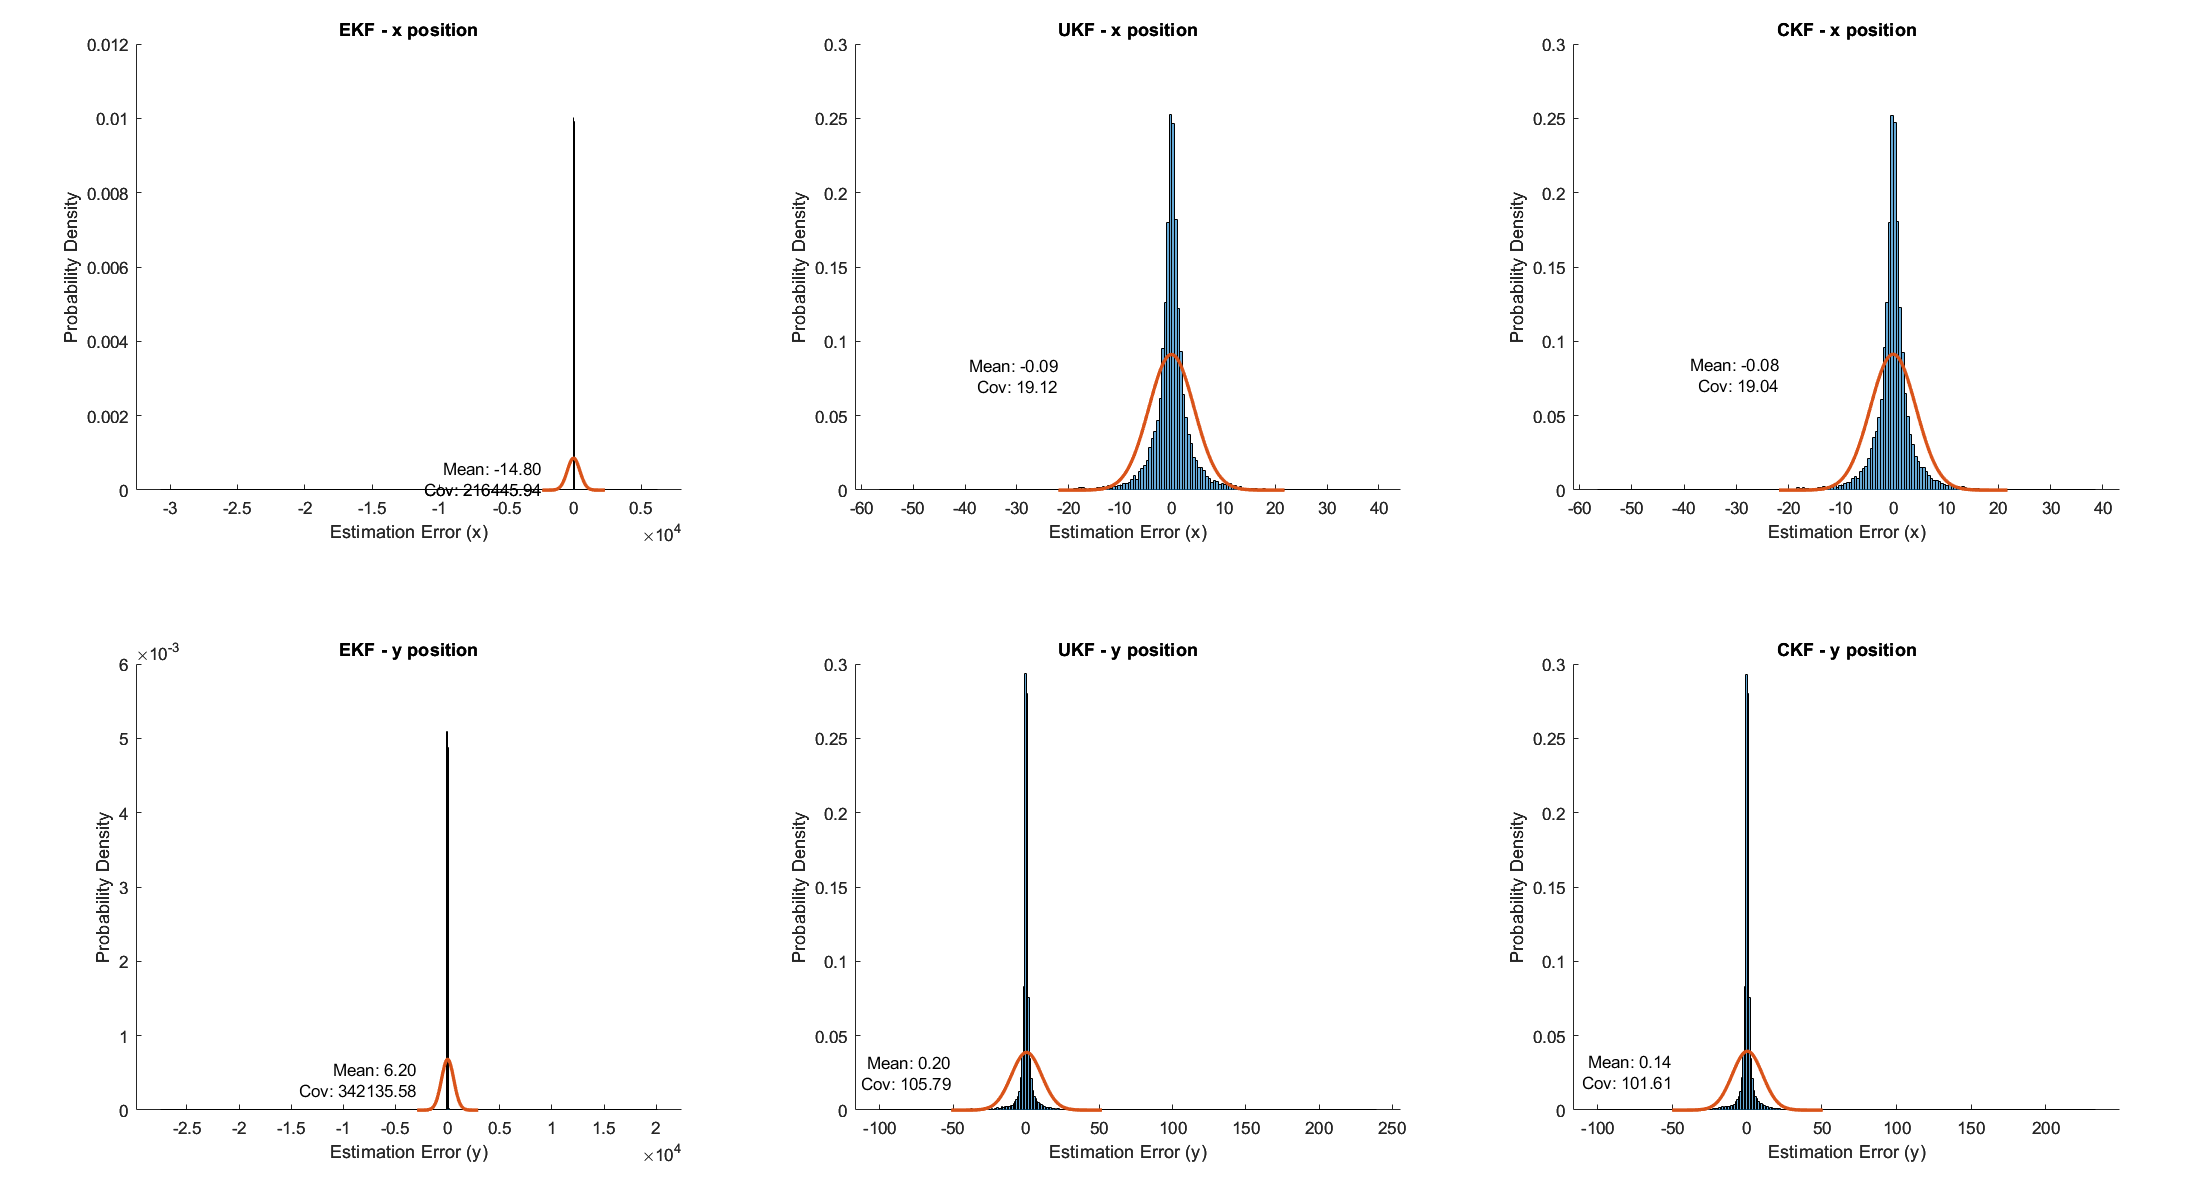
\includegraphics[width=0.95\textwidth]{images/hiscase3.png}
 \caption{Case 3}
 \label{c3}
\end{figure}

From figures above, concentrate on the Mean value ( the closer to zero, the better the quality), we can see that EKF has the worst performance within three methods, while the UKF and the CKF has nearly the same performance. 

The histogram of EKF has nothing bussiness with Gaussian distribution, and that explains why its mean so far away from zero. From the histograms of UKF and CKF, we can see the histograms for $ x $ look quite like Gaussian. But when turns to y, since it is a nonlinear measurement model, the more the nonlinear, the less the histograms look like Gaussian.

And the normalpdf curves are drawn within the  $ \pm 5 \sigma $, since from the figures in Task a we can see the measurement points are so scattered that the nosies are too big, which leads to many points do not lie within the $ \pm 5 \sigma $ zone. So even with normalization, the curve can only looks quite like Gaussian but not coincident to it like the previous homeworks.